\chapter{Описание пользовательских интерфейсов системы}
Пользовательские интерфейсы построены на базе веб-технологий с помощью языка разметки HTML.
Для стилизации интерфейса был задействован фронт-енд фреймоворк Bootstrap.
Видеопотоки проигрываются с помощью мультимедиа плеера VLC, встроенного в браузер через плагин.
Для обеспечения динамичности интерфейса была задействована javascript библиотека jQuery.

\begin{figure}[!htb]
\def\svgwidth{\columnwidth}
\center{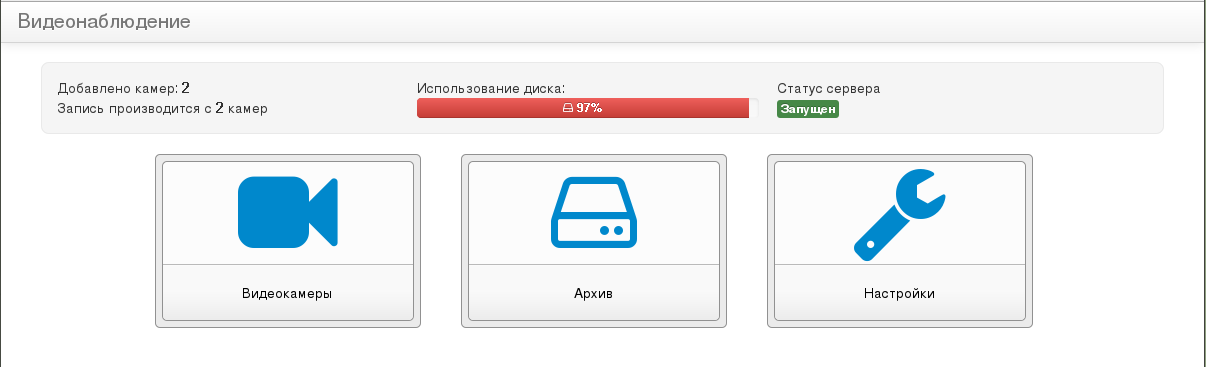
\includegraphics[width=0.8\linewidth]{img/ui_1_main.png}}
\caption{}
\label{ui_1}
\end{figure}

\section{Главная страница системы}
Пример главной страницы представлен на рис.\ref{ui_1}.

Главная страница предоставляет информацию о параметрах работы системы и содержит
кнопки для перехода к другим модулям.

В блоке информации о параметрах работы системы отображается:
\smallskip
\begin{itemize}
\item количество добавленных в систему камер
\item количество камер, с которых видеосервер производит запись в настоящее время
\item процент использования дискового пространства
\item статус видеосервера
\end{itemize}

Данная информация получается от модуля работы с графическим интерфейсом видеосервера
в результате отправки специального json запроса через unix сокет.

\begin{itemize}
\item Кнопка <<Видеокамера>> позволяет перейти к интерфейсу выбора камер для просмотра.
\item Кнопка <<Архив>> позволяет перейти к интерфейсу просмотра архивных видеозаписей, информации
о произошедших событиях и созданных видеофайлах.
\item Кнопка <<Настройки>> позволяет перейти к интерфейсу настроек видеокамер.
\end{itemize}

\section{Страница настроек видеокамер}
Пример страницы настроек видеокамер представлен на рис.\ref{ui_6}.

На странице отображается таблица добавленных в систему видеокамер.
Для каждой камеры имеется возможность перехода к странице информации о видеокамере,
странице редактирования настроек камеры и имеется кнопка удаления камеры из системы.

\begin{figure}[!htb]
\def\svgwidth{\columnwidth}
\center{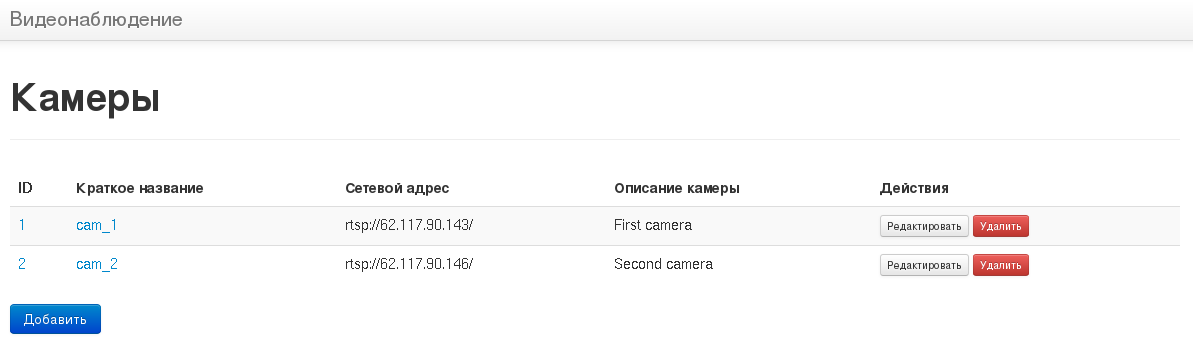
\includegraphics[width=0.8\linewidth]{img/ui_6_cameras.png}}
\caption{}
\label{ui_6}
\end{figure}

\section{Страница создания/редактирования видеокамеры}
Пример страницы создания/редактирования видеокамеры представлен на рис.\ref{ui_4}.

Страница содержит форму для заполнения данных видеокамеры.
При сохранении производится валидация данных:
\smallskip
\begin{itemize}
\item проверяется заполнение обязательных полей
\item производится проверка на максимальную длину вводимых данных
\item проверяется корректность адреса камеры
\item проверяется уникальность краткого названия
\end{itemize}

\section{Страница просмотра информации о видеокамере}
Пример страницы просмотра информации о видеокамере представлен на рис.\ref{ui_5}.
Страница содержит информацию о настройках камеры, введенных пользователем, и информацию
о видеопотоке, передаваемым камерой (разрешение, частота кадров, кодек).
Информацию о видеопотоке предоставляет по запросу видеосервер.
Также страница содержит изображение кадра с камеры, который обновляется один раз в минуту.

\newpage

\begin{figure}[!htb]
\def\svgwidth{\columnwidth}
\center{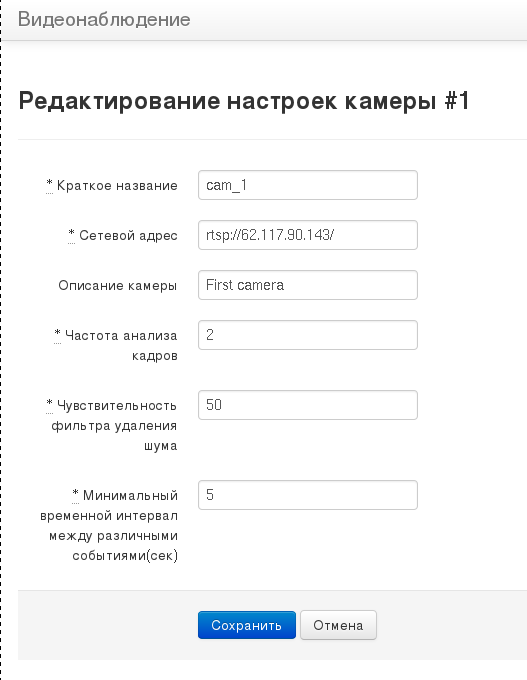
\includegraphics[width=0.6\linewidth]{img/ui_4_settings.png}}
\caption{}
\label{ui_4}
\end{figure}

\begin{figure}[!htb]
\def\svgwidth{\columnwidth}
\center{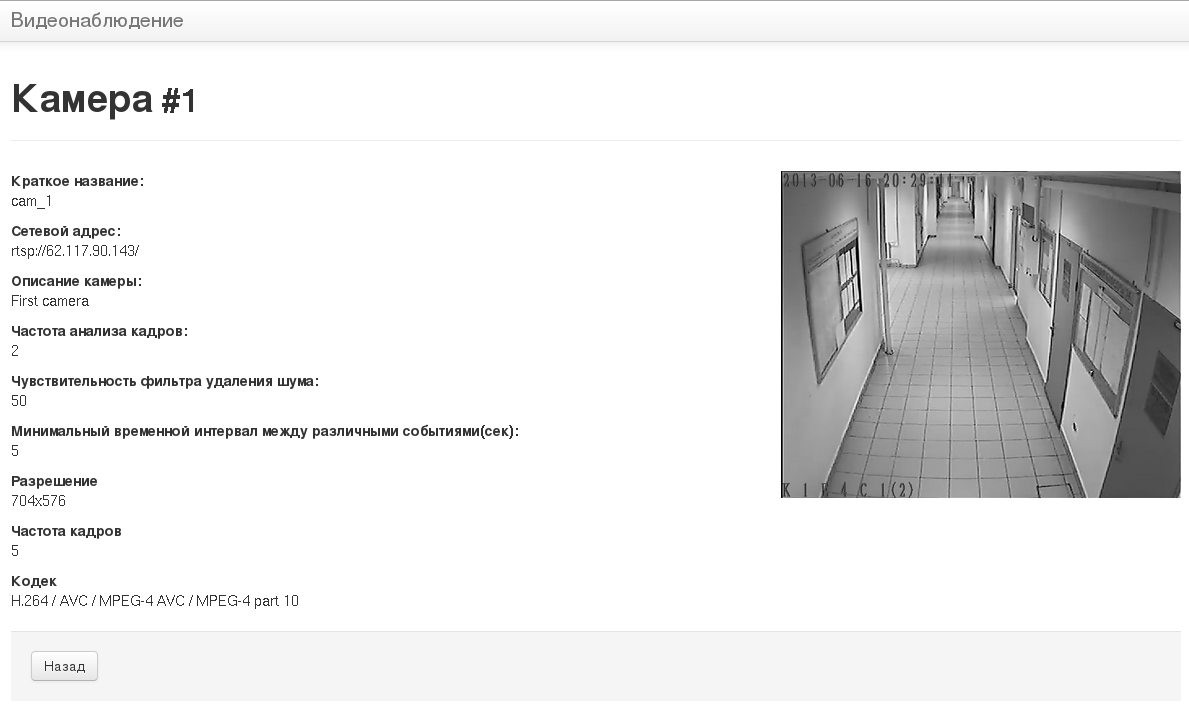
\includegraphics[width=0.8\linewidth]{img/ui_5_show.png}}
\caption{}
\label{ui_5}
\end{figure}

\newpage

\section{Страница выбора камер для просмотра}
Пример страницы выбора камер для просмотра представлен на рис.\ref{ui_2}.

Сначала выбирается количество одновременно показываемых камер.
Затем выбираются желаемые камеры.
Интерфейс также позволяет по принципу drag\&drop упорядочить камеры в
произвольном порядке. Данный порядок сохраняется в базе данных и не
утрачивается между сеансами.

\begin{figure}[!htb]
\def\svgwidth{\columnwidth}
\center{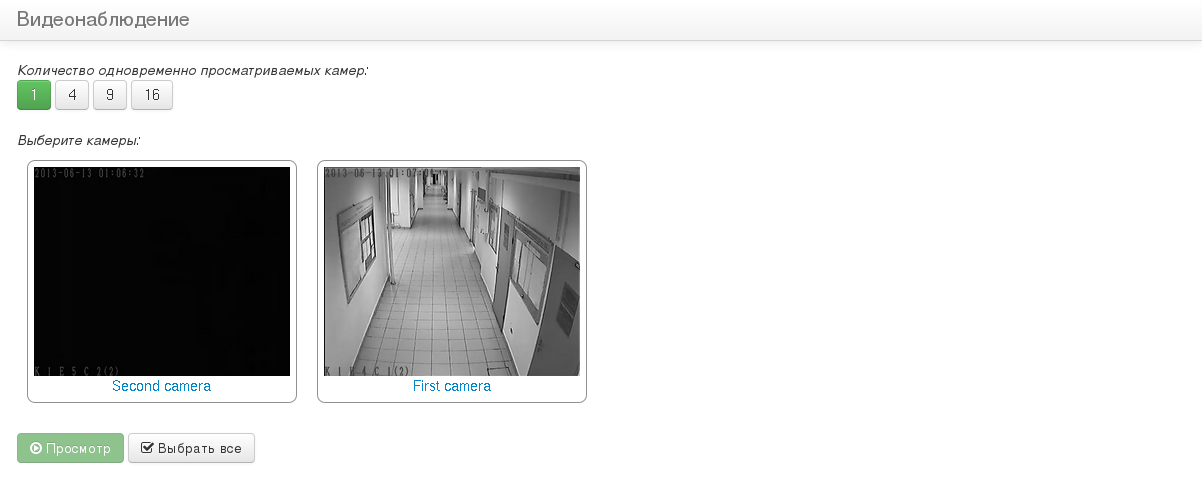
\includegraphics[width=0.8\linewidth]{img/ui_2_select.png}}
\caption{}
\label{ui_2}
\end{figure}

\section{Страница просмотра архива видеокамеры}
Пример страницы просмотра архива видеокамеры представлен на рис.\ref{ui_3}.

На данной странице можно просмотреть видеозапись любого момента времени.
С помощью календаря осуществляется выбор желаемого дня. Информация о событиях и произведенных
видеозаписях подгружается с помощью AJAX без перезагрузки страницы и без остановки просмотра
текущей видеозаписи.

Все произведенные видеозаписи и произошедшие события отображаются на временной ленте.
Лента показывает информацию об одном дне. Синими полосами отмечаются интервалы времени,
для которых доступны видеозаписи. Оранжевые полосы~-- интервалы времени, в которые было обнаружено
движение.

При наведении указателя на временную полосу, снизу отображается соответствующее время суток.
Щелчок по временной полосе включает показ видеозаписи с данного момента времени.
При необходимости, можно увеличить масштаб временной ленты.
Это позволит более точно выбрать момент времени.
При увеличении масштаба становится активна полоса прокрутки временной ленты.

\begin{figure}[!htb]
\def\svgwidth{\columnwidth}
\center{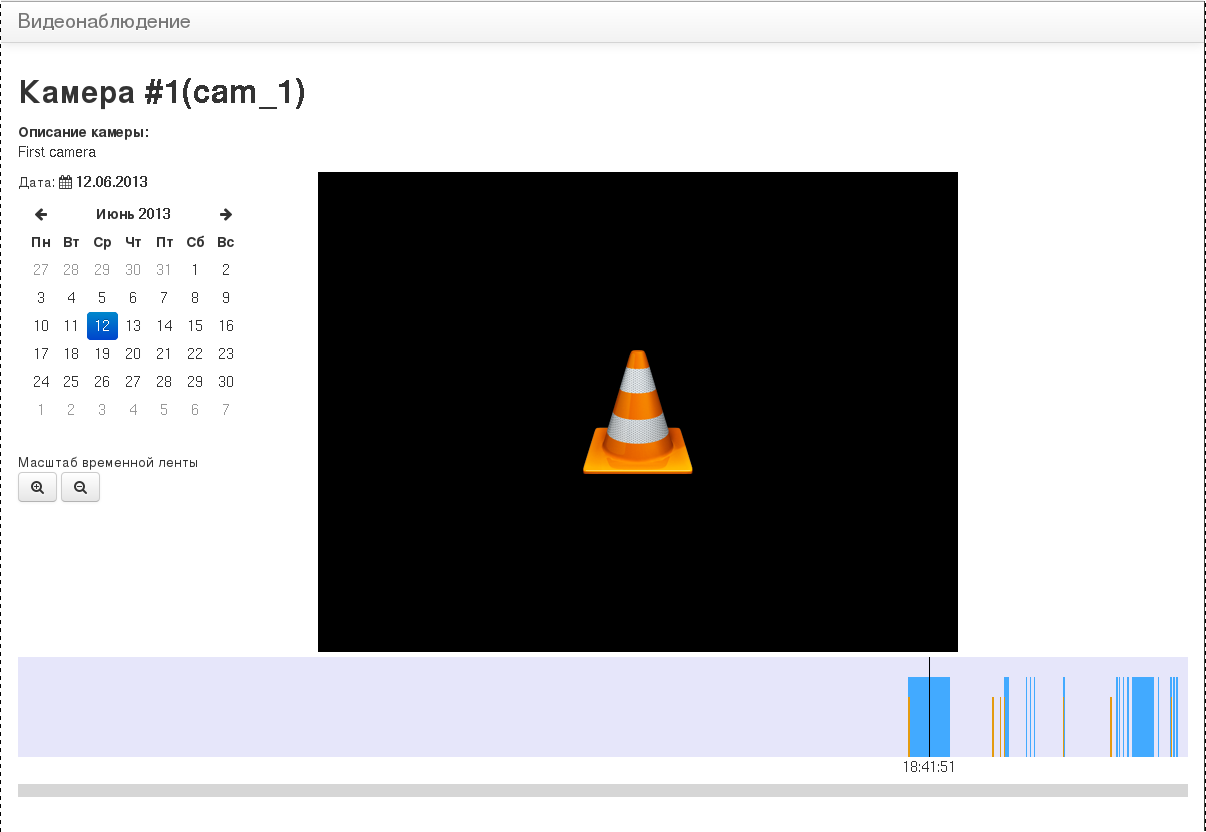
\includegraphics[width=0.8\linewidth]{img/ui_3_archive.png}}
\caption{}
\label{ui_3}
\end{figure}
